\section{Theorie}
\label{sec:Theorie}

\subsection{Reflexion und Brechungsindex}
\label{theo1}

Trifft Röntgenstrahlung aus dem Vakuum auf ein Medium mit einem Brechungsindex $n \neq 1$ ist der Brechungsindex gegeben als
\begin{equation}
    n = 1 −  \delta + i \cdot \beta \,.
    \label{eq:index}
\end{equation}
Dabei ist $\delta$ eine kleine Korrektur $\delta = 10^(-6)$ und $\beta$ die Absorption.
Für Röntgenstrahlen ist der Brechungsindex in Materie kleiner als 1, sodass Totalrelflexion möglich wird.
Zunächst betrachten wir allerdings eine allgemeine Reflexion.
Eine elektromagnetische Welle trifft unter einem Winkel $\alpha_\text{i}$ auf eine homogene, unendlich dicke und glatte Schicht.
Dort wird ein Teil der Welle unter dem Winkel $\alpha _\text{f} = \alpha _\text{i}$ reflektiert und der andere Teil um den Winkel $\alpha _\text{f}$ transmittiert und gebrochen.
Die Reflexion und Transmission ist in \autoref{fig:theo1} dargestellt.

\begin{figure}
    \centering
    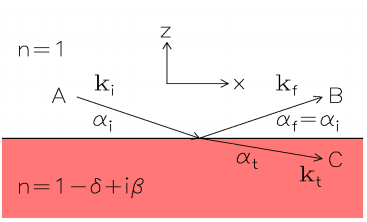
\includegraphics[width=0.5\textwidth]{images/reflektion.png}
    \caption{Darstellung der Reflexion und Transmission einer Welle. \cite{V44-old}}
    \label{fig:theo1}
\end{figure}

Wie bereits besprochen ist hier unterhalb eines bestimmten kritischen Winkels $\alpha _\text{c}$ Totalrelflexion möglich, das bedeutet, dass kein Teil der Welle transmittiert wird.
Dieser Winkel ist näherungsweise gegeben durch
\begin{equation}
    \alpha _\text{c} = \sqrt{2 \cdot \delta} \,.
    \label{eq:krit}
\end{equation}
Wird nun die Definition von $\delta$ verwendet, ergibt sich $\alpha _c$ als 
\begin{align}
    \delta &= \frac{\lambda ^2 \cdot r_\text{e} \cdot \rho}{2 \, \pi} \\
    \alpha _\text{c} &=  \lambda  \cdot \sqrt{\frac{r_\text{e} \cdot \rho}{\pi}} \,.
\end{align}

In den Fresnelschen-Gleichungen wird zudem die Polarisation der Wellen betrachtet.
Da beide $n$ im Falle von Röntgenstrahlung nahezu gleich sind, ist die Polarisation in den Fresenl-Gleichungen zu vernachlässigen.
Dadurch haben beide Polarisationen die Form
\begin{align}
    t &= \frac{2 \, N_1 \, \sin{\alpha _\text{i}} }{N_1 \, \sin{\alpha _\text{i}} + N_2 \, \sin{\alpha _\text{t}}} \\
    r &= \frac{N_1 \, \sin{\alpha _\text{i}} - N_2 \, \sin{\alpha _\text{t}}}{N_1 \, \sin{\alpha _\text{i}} + N_2 \, \sin{\alpha _\text{t}}} \,.
\end{align}
Dabei sind $r$ und $t$ die Fesnel'schen Reflexions- und Transmissionskoeffizienten. 
Diese stellen Amplitudenverhältnisse dar, allerdings wir sind eher an Intensitätsverhältnissen interessiert.
Daher betrachten wir die Fresnel'sche Reflektivität unter der Annahme, dass $\alpha _\text{i} > 3 \, \alpha _\text{c}$ als 
\begin{equation}
    R_\text{F} = |r|^2 = \left( \frac{{\alpha _\text{c}}^4}{2 \, \alpha _\text{i}}  \right) \,.
    \label{eq:reflek}
\end{equation}

\subsection{Mehrschichtsysteme}
\label{theo2}

In der Realitiät sind Systeme aber selten homogen und einschichtig, daher wird zunächst die Reflexion an einer Probe mit Schicht untersucht.
Als Beispiel soll ein Silizium-Wafer mit einer $\SI{800}{\angstrom}$ dicken Polystyrolschicht dienen. 
Trägt man die Reflektivität gegen den Einfallswinkel auf ergibt sich ein Plot wie in \autoref{fig:theo2}.

\begin{figure}
    \centering
    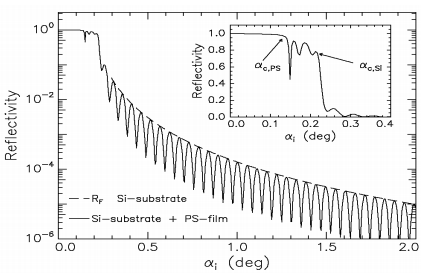
\includegraphics[width=0.5\textwidth]{images/plot.png}
    \caption{Reflektivität in Abhängigkeit vom Einfallswinkel bei unserem Beispiel. \cite{V44-old}}
    \label{fig:theo2}
\end{figure}

Die gestrichelte Linie stellt die theoretische Fresnelreflektivität dar.
Es ist allerdings zu erkennen, dass sie in der Realität oszilliert, dies sind die sogenannten Kiessig-Oszillazionen. 
Sie entstehen durch Interferenz an den Grenzflächen, die je nach Phasendifferenz konstruktiv oder destruktiv ist.
Die Minima entstehen, wenn sich zwei Wellen auslöschen, das geschieht bei einem Gangunterschied von $ n \cdot \frac{\lambda}{2}$, wobei $n$ eine ungerade Zahl ist.
Bei den kritischen Winkeln beider Schichten sind klare Einbrüche im Plot zu erkennen. 
So ergeben sich die Winkel
\begin{align}
    \alpha _\text{c,PS} &= \SI{0.15}{\degree} \\
    \alpha _\text{c,SI} &= \SI{0.22}{\degree}
\end{align}
aus dem Plot.
Über die Wellenlänge $\lambda$ der Oszillazion kann die Schichtdicke $d$ als 
\begin{equation}
    d = \frac{\lambda}{2 \, \Delta \alpha _\text{i}}
    \label{eq:schicht}
\end{equation}
berechnen werden.

Sollte es noch weitere Schichten geben, werden die Oszillazionen überlagert und es ist kompliziert etwas über die einzelnen Schichten auszusagen.
Dafür gibt es den sogenannten Parrat-Algorithmus, dieser basiert auf einem rekursiven Durchlaufen durch alle Schichten.
Angefangen wird dabei mit der untersten Schicht.
Es werden dabei die Amplitudenverhältnisse der jeweils j-ten Schicht untersucht.
Der Algorithmus wird durch 
\begin{equation}
    X_\text{j} =  \exp(-2 i k_\text{z,j} z_\text{j}) \cdot  \frac{r_\text{j,j+1} + X_\text{j} \exp(-2 i k_\text{z,j+1} z_\text{j})}
    {1 + r_\text{j,j+1} X_\text{j} \exp(-2 i k_\text{z,j+1} z_\text{j})}
    \label{eq:parratt}
\end{equation}
beschrieben.
Hierbei ist
\begin{equation}
    k_\text{z,j} = k \cdot \sqrt{n_\text{j}^2 -  {\cos{\alpha _\text{i}}}^2}
    \label{eq:k}
\end{equation}
die $z$-Komponente des j-ten Wellenvektors und 
\begin{equation}
    r_\text{j,j+1} = \frac{k_\text{z,j} - k_\text{z,j+1}}{k_\text{z,j} + k_\text{z,j+1}} \,.
    \label{eq:k}
\end{equation}


Eine weitere Korrektur ist noch nötig, die Rauigkeitskorrektur. 
Glatte Oberflächen treten in der Natur nicht wirklich auf, daher wird eine "root-mean-square“ (rms) – Rauigkeit der j-ten Grenzfläche eingeführt.
Mit Hilfe dieser werden die Fresnelkoeffizienten modifiziert.
Diese können dann im Parratt-Algorithmus verwendet werden, ansonsten bleibt die Rechnung die gleiche.

\subsection{Funktionsweise der Geräte im Versuch}
\label{theo3}
 
Die Röntgenstrahlung erhalten wir aus einer Kupfer-Röntgenröhre.
Dort werden Elektronen aus einer Glühkathode gelöst und dann zu einer Kupferanode beschleunigt, dort geben sie Bremsstrahlung ab.
Durch Stöße mit den Hüllenelektronen entsteht außerdem die charakteristische Strahlung.
Für diesen Versuch wird die charakteristische $K_\text{\alpha}$ von Kupfer für die Reflektometrie verwendet.
Damit auch nur diese für die Reflektometrie benutzt wird, trifft die Strahlung auf einen Göbelspiegel.
Dort wird die Strahlung zudem monochromatisiert und gebündelt, sodass die Strahlen nun parallel verlaufen.
Das von dort kommende Licht besitzt nun eine Wellenlänge von $\lambda = \SI{1.54}{\angstrom}$, was der $K_\text{\alpha}$ von Kupfer entspricht.
Nach einer Abschwächung der Intensität durchläuft der Strahl eine Blende, diese definiert den Einfallswinkel $\alpha_\text{i}$.
Idealerweise trifft die Röntgenstrahlung auf die Probe und wird zum Detektor hin reflektiert.
Vor dem Detektor befindet sich ebenfalls eine Blende, die den Ausfallswinkel $\alpha_\text{f}$ definiert.

Allerdings gibt es eine zusätzliche Bedingung für den Einfallswinkel.
Erst ab einem genügend großen Winkel $\alpha_\text{g}$ wird der gesamte Strahl tatsächlich reflektiert.
Dafür wird der Geometriefaktor $G$ 
\begin{equation}
    G = \frac{D \cdot \sin{\alpha _\text{i}}}{d_\text{0}}
    \label{eq:geo}
\end{equation}
definiert.
Dabei ist $d_\text{0}$ die Gesamtstrahlbreite und $D \cdot \sin{\alpha _\text{i}}$ die Strahlbreite, die tatsächlich auf die Probe trifft.
Damit wäre ein $G$ von 1 optimal, allerdings wird das in diesem Versuch nicht immer realisiert.
